%%
%% FatecTeX: A class for academic works (undergraduate thesis, monographs, and reports)
%% Faculty of Technology of Pompéia (FATEC Pompéia), Brazil
%%
%% Version 1.0.0 2025/08/17
%% Copyright (C) 2025 
%% 
%% Modified and adapted by Prof. Dr. Cássio Faria da Silva (FATEC Pompéia)
%% <cassiofs@gmail.com>
%% from the fatectex class originally developed for the University of Brasília (UnB)
%% by Henrique C. Ferreira <hcferreira@unb.br>
%%
%% This class file may be distributed and/or modified under the conditions
%% of the LaTeX Project Public License, either version 1.3 of this license,
%% or (at your option) any later version.
%% The latest version of this license is available at:
%%
%%    https://www.latex-project.org/lppl.txt
%%
%% and version 1.3 or later is part of all LaTeX distributions
%% released 2005/12/01 or later.
%%
%% ------------------------------------------------------------------------
%% This file is a template for use with FatecTeX
%% To compile the document you should run: pdflatex, bibtex, pdflatex
%% ------------------------------------------------------------------------


\documentclass[
    % -- Opção da classe memoir -- https://www.ctan.org/pkg/memoir
    oneside, % Para imprimir somente na frente da folha
    %twoside, % Para imprimir na frente e no verso da folha
    % -- Opção da classe abntex2 -- https://www.ctan.org/pkg/abntex2
    sumario=tradicional, % Remova esta opção para sumário padrão ABNT
    % -- Selecione o idioma no qual o trabalho será escrito
    idioma=brazil, % Para texto principal em português
    %idioma=english, % Para texto principal em inglês  
    % -- Selecione o estilo das referências bibliográficas
    bib=alf, % Bibliografia nas normas da ABNT, estilo autor-data
    %bib=num, % Bibliografia nas normas da ABNT, estilo numérico
    % -- Selecione o estilo de numeração de figuras, tabelas, etc.
    numb=chap, % Numeração por capítulo
    %numb=abnt, % Numeração para o documento inteiro
    ]{fatectex}

% ---
% Pacotes básicos (Adicione outros pacotes necessários para o seu trabalho)
% ---
\usepackage{lscape} % Pacote para rotacionar tabelas (e outros objetos)
%\usepackage{pdflscape} % Pacote para rotacionar objetos e também a página do arquivo pdf
\usepackage{afterpage} % Evita quebra de página quando inserir uma tabela (ou outro objeto) rotacionada
% ---

% ---
% Compila a nomenclatura
% ---
\makenomenclature
% ---

% ---
% Diretório das figuras
\graphicspath{{fatectex-example/figuras}}
% --- 

% ------------------------------------------------------------------------
% ------------------------------------------------------------------------
% Informações do trabalho
% ------------------------------------------------------------------------
% ------------------------------------------------------------------------

% ---
% Título
% ---
\titulo{Projeto Integrador de\\Sistemas Inteligentes II} % No idioma principal do texto
% Insira \\ caso queira forçar quebras de linha no título
% Não utilize caixa alta para o título do trabalho e nem das seções (com exceção de siglas)
% ---
\tituloestrangeiro{} % Escreva aqui título em português se o trabalho for escrito em inglês (caso contrário, deixe vazio)
% ---

% ---
% Autores
% ---
%\autori[]{Peter}{Benjamin Parker} % \autori[]{Nome}{Sobrenome} 
\autori[]{Leia Organa Skywalker \\ Peter Benjamin Parker \\ Daenerys Stormborn Targaryen}{}
% No caso de nomes como Carlos de Souza, utilize \autori[]{Carlos de}{Souza} (e não \autori[]{Carlos}{de Souza})
% ---
\autorii[]{}{} % Deixe os argumentos vazios se não tiver segundo autor
% ---

% ---
% Código Cutter para a ficha catalográfica
% Gerado a partir da entrada <Sobrenome, Nome> (do primeiro autor) no site https://www.tabelacutter.com/
% ---
\numerocutter{} % Para não imprimir o código na ficha catalográfica, deixe o argumento vazio
%\numerocutter{769} % Prencher o argumento do comando apenas com os números gerados
% ---

% ---
% Orientadores
% ---
\orientador[Orientador]{Prof. Dr.}{Thomas Alva Edison}{FATEC - Pompéia} % Para alterar o gênero, basta trocar Orientador por Orientadora
% ---
\coorientador[Coorientador]{Prof. Dr.}{}{} % Deixe os argumentos para nome e sobrenome vazios se não tiver coorientador 
% ---

% ---
% Informações do curso
% ---
\tipotrabalho{Projeto de Extensão} % Projeto de Extensão; Dissertação de Mestrado; Tese de Doutorado (em português, mesmo que o trabalho seja em inglês)
% ---
\tipocurso{Temática: Ações de ciência, tecnologia e inovação} % Nome do curso de graduação ou do programa de pós-graduação, em português
% Ou ainda a temática: Temática: Ações de ciência, tecnologia e inovação
%\tipocurso{Programa de Pós-Graduação em Engenharia Elétrica}
% ---
% Texto que aparece na folha de rosto e na folha de aprovação
\preambulo{Projeto de Extensão Universitária submetido como requisito parcial para promoção na disciplina de Projeto Integrador de Sistemas Inteligentes II}
%\preambulo{Trabalho de Conclusão de Curso submetido como requisito parcial para obtenção do grau de Engenheiro Eletricista.} 
%\preambulo{Tese de Doutorado submetida ao Programa de Pós-Graduação em Engenharia Elétrica da Universidade de Brasília como parte dos requisitos necessários para obtenção do grau de Doutor.}
% Consulte a secretaria/coordenação do curso para saber o que deve ser escrito no preâmbulo. Use português mesmo que o trabalho seja em inglês.
% ---
% Informação adicional para ser impressa na folha de rosto
\publicacao{} % Deixe o argumento vazio caso não haja
%\publicacao{Publicação PPGEE 201/23} % Também imprime as informações do trabalho no topo da página da ficha catalográfica
% ---

% ---
% Instituição
% ---
\instituicao[Centro Paula Souza -- CEETPS]{FATEC Pompeia - Shunji Nishimura}{Tecnologia em Sistemas Inteligentes} % Caso queira incluir o departamento da unidade acadêmica
% ---

% ---
% Local e data da defesa
% ---
\local{Pompéia}
\dia{}
\mes{}
\ano{2025}
% ---

% ---
% Membros da banca
% ---
\membrodabancai{Prof. Dr. Albert Einstein,\\ FATEC - Pompéia} % Membro 1 - Geralmente é o orientador
\membrodabancaifuncao{Orientador} % Em português, mesmo que o trabalho seja em inglês.
\membrodabancaii{Profa. Dra. Ada Lovelace,\\ FATEC - Pompéia} % Membro 2
\membrodabancaiifuncao{Examinador interno}
\membrodabancaiii{Prof. Dr. Alan Mathison Turing,\\ FATEC - Pompéia} % Membro 3
\membrodabancaiiifuncao{Examinador interno}
\membrodabancaiv{} % Deixe vazio se não tiver o quarto membro
\membrodabancaivfuncao{Examinador externo}
\membrodabancav{} % Deixe vazio se não tiver o quinto membro
\membrodabancavfuncao{Examinador externo}
% Comprimento da linha da assinatura (ajuste conforme necessidade)
\signlinewidth{9cm}
% ---

% ---
% Resumo em português
% ---
\begin{Resumo}
Até 250 palavras: problema, ODS, método, solução, principais resultados/entregas.

Palavras-chave: 3–5 termos.

Exemplo didático
Resumo: “Este projeto aborda a automatização da triagem de resíduos recicláveis (ODS 12) para a Cooperativa Verde. Utilizou-se uma arquitetura de dados com coleta via app móvel, armazenamento em banco relacional e modelo de visão computacional (Random Forest + SIFT). A solução incrementou em 18\% a precisão da triagem piloto. Entregas: dataset, API de classificação, dashboard e manual.”
\end{Resumo}
% ---

% ---
% Resumo em inglês
% ---
\begin{Abstract}
Aqui a versão em inglês...
\end{Abstract}
% ---

% ---
% Palavras-chave (defina no mínimo 3 e no máximo 5)
% ---
\pchavei{palavra-chave 1}
\kwordi{keyword 1}
\pchaveii{palavra-chave 2}
\kwordii{keyword 2}
\pchaveiii{palavra-chave 3}
\kwordiii{keyword 3}
\pchaveiv{palavra-chave 4} % Deixe vazio se não tiver
\kwordiv{keyword 4} % Deixe vazio se não tiver
\pchavev{} % Deixe vazio se não tiver
\kwordv{} % Deixe vazio se não tiver
% ---

% ---
% Agradecimentos
% ---
% Idioma usado nos agradecimentos (pode ser em português, mesmo que o trabalho seja em inglês)
\idiomaagradecimentos{brazil}
%\idiomaagradecimentos{english}

\begin{otherlanguage*}{\acklang}

% Primeiro autor
% Quando se tem até dois autores, é possível criar uma seção para cada um
\begin{AgradecimentosAutorI}
Nesta seção, o autor deve registrar seus agradecimentos formais a todas as pessoas e instituições que contribuíram, direta ou indiretamente, para a realização do trabalho acadêmico. É comum mencionar orientadores, professores, colegas, familiares e agências de fomento, destacando o apoio recebido ao longo da pesquisa e do processo de formação.

O texto deve ser redigido de maneira clara, objetiva e em tom respeitoso, evitando exageros ou informalidades. Não existe um tamanho fixo, mas recomenda-se que seja breve e conciso, ocupando normalmente de um a três parágrafos. Este espaço é opcional, porém representa uma oportunidade de valorizar a colaboração daqueles que auxiliaram na trajetória acadêmica do autor.
\end{AgradecimentosAutorI}

% Segundo autor
\begin{AgradecimentosAutorII}
Agradecimentos do segundo autor.
\end{AgradecimentosAutorII}

\end{otherlanguage*}
% ---

% ---
% Dedicatória
% ---

% Primeiro autor
\begin{DedicatoriaAutorI}
Este trabalho é dedicado às crianças adultas que,\\
quando pequenas, sonharam em se tornar cientistas.
\end{DedicatoriaAutorI}

% Segundo autor
\begin{DedicatoriaAutorII}
Dedicatória do segundo autor.
\end{DedicatoriaAutorII}
% ---

% ---
% Epígrafe
% ---
\begin{Epigrafe}
\vspace*{\fill}
\begin{flushright}
    \textit{``If you find that you're spending almost all your time on theory,\\
    start turning some attention to practical things;\\
    it will improve your theories.\\
    If you find that you're spending almost all your time on practice,\\
    start turning some attention to theoretical things;\\
    it will improve your practice.''\\
    (Donald Knuth)}
\end{flushright}
\end{Epigrafe}
% ---

% ------------------------------------------------------------------------
% ------------------------------------------------------------------------
% Início do documento
% ------------------------------------------------------------------------
% ------------------------------------------------------------------------
\begin{document}

% ------------------------------------------------------------------------
% ELEMENTOS PRÉ-TEXTUAIS
% ------------------------------------------------------------------------
\pretextual
% ------------------------------------------------------------------------

% Insere capa e contracapa
\imprimircapa

% Insere folha de rosto
\imprimirfolhaderosto*

% Insere ficha bibliográfica
%\fichacatalografica

% Insere folha de aprovação
%\imprimirfolhadeaprovacao

% Insere dedicatória (elemento opcional)
%\imprimirdedicatoria

% Insere agradecimentos (elemento opcional)
%\imprimiragradecimentos

% Insere epígrafe (elemento opcional)
%\imprimirepigrafe

% Insere resumos
\imprimirresumos

% Insere lista de figuras
%\imprimirlistadefiguras

% Insere lista de quadros
%\imprimirlistadequadros

% Insere lista de tabelas
%\imprimirlistadetabelas

% Insere lista de algoritmos
%\imprimirlistadealgoritmos

% Insere lista de códigos
%\imprimirlistadecodigos

% Insere a lista de abreviaturas e siglas e a lista de símbolos
\imprimirlistadesiglasesimbolos

% Insere o sumário
\imprimirsumario

% ------------------------------------------------------------------------
% ELEMENTOS TEXTUAIS
% ------------------------------------------------------------------------
\textualsimples % Cabeçalho com número da página e linha horizontal
%\textual % Cabeçalho com número da página, título do capítulo/seção e linha horizontal
% ------------------------------------------------------------------------

% Imprime uma página para agrupar um conjunto de capítulos (parte)
%\part{Nome da parte}

% Capítulo de introdução
% ----------------------------------------------------------
\chapter{Introdução}
\label{cap:intr}
% ----------------------------------------------------------

Desenvolver um trabalho prático baseado em problema que integre as teorias abordadas nas disciplinas do 1º semestre. Este trabalho precisa ser baseado em uma necessidade tecnológica de uma organização real, ou deve colaborar com um dos Objetivos de Desenvolvimento Sustentáveis (ODS) da Organização das Nações Unidas (ONU) voltando-se no auxílio direto para a sociedade.

O trabalho a ser desenvolvido consiste em desenvolver projetos para coleta, gerenciamento e processamento de dados por meio de algoritmos computacionais.


% ----------------------------------------------------------
\chapter{Caracterização do Projeto}
\label{cap:caracterizacao}
% ----------------------------------------------------------

Nesta seção são apresentados os elementos fundamentais que compõem a estrutura do projeto de extensão, fornecendo uma visão inicial sobre sua organização, abrangência e público de interesse. O objetivo é contextualizar a proposta, destacando os aspectos centrais que orientam sua execução e justificam sua relevância para a comunidade acadêmica e externa.

São descritos a seguir a carga horária prevista, o público-alvo, o parceiro e stakeholders envolvidos, bem como o diagnóstico inicial que fundamenta a necessidade e pertinência da iniciativa. Essas informações permitem compreender a dimensão do projeto e estabelecer a base para o desenvolvimento das atividades planejadas.

\section{Carga horária}

Um total de 80 horas/aula será aplicado na disciplina Projeto Integrador II, integrado com os demais componentes curriculares do 2º semestre.

\section{Público-alvo}

Organizações, empresas, associações e organizações não governamentais parceiras da Fatec.

\section{Parceiro, Stakeholders e Diagnóstico Inicial}

\begin{itemize}
    \item Organização parceira: missão, processos relevantes, dados disponíveis.
    \item Stakeholders: quem usa, quem decide, quem mantém (matriz RACI opcional).
    \item Restrições: orçamento, prazos, infraestrutura, LGPD/ética.
\end{itemize}

Exemplo:

Parceiro: Cooperativa Verde (80 colaboradores)...

Stakeholders: triadores (U), gerente (A), TI municipal (C), equipe do projeto (R)...

Restrições: sem internet no galpão; dados sensíveis (biometria NÃO coletada)...



% Capítulo de objetivos
% ----------------------------------------------------------
\chapter{Objetivos}
\label{cap:objetivos}
% ----------------------------------------------------------

Possibilitar o desenvolvimento das competências profissionais e socioemocionais. Melhorar a integração dos discentes com as organizações atendidas pelo projeto, por meio do desenvolvimento de um artefato tecnológico.

\section{Objetivo Geral}

\begin{itemize}
    \item Possibilitar o desenvolvimento de competências profissionais e socioemocionais dos discentes, melhorando a integração com organizações atendidas pelo projeto e promovendo o desenvolvimento de um artefato tecnológico.
\end{itemize}


\section{Objetivos Específicos}

\begin{itemize}
    \item Identificar problemas reais em organizações parceiras relacionados aos ODS da ONU.
    \item Analisar requisitos e cenários para o desenvolvimento de soluções tecnológicas.
    \item Desenvolver algoritmos de processamento e conexão de dados em ambientes computacionais.
    \item Avaliar resultados e propor melhorias para os sistemas desenvolvidos.
    \item Elaborar documentação técnica e científica detalhando as soluções e metodologias aplicadas.
\end{itemize}



% Capítulo com a metodologia
% ----------------------------------------------------------
\chapter{Metodologia}
\label{cap:metodologia}
% ----------------------------------------------------------

O projeto será desenvolvido em grupos de trabalho e dividido nas seguintes etapas:

Definição do problema: 

\begin{enumerate}
    \item Identificação de tema e problema vinculado aos ODS da ONU ou desafios propostos por organizações parceiras, com suporte do professor orientador.
    \item Levantamento de requisitos: Análise detalhada do cenário do desafio, identificando as necessidades da organização.
    \item Modelagem da solução: Desenvolvimento de arquitetura para armazenamento e processamento de dados.
    \item Implementação de algoritmos: Criação de algoritmos de conexão, análise e processamento de dados.
    \item Avaliação dos resultados: Testes e validação da solução desenvolvida frente ao problema identificado.
    \item Documentação: Elaboração de relatórios técnicos e artigos científicos detalhando todas as etapas e resultados.
    \item Apresentação: Comunicação dos resultados para as partes interessadas do projeto, incluindo a organização parceira.
\end{enumerate}


\section{Ferramentas e técnicas utilizadas}

\begin{itemize}
    \item Figma, Adobe XD, Sketch ou outra ferramenta de design de interfaces digitais (UI/UX).
    \item Python, R ou outra linguagem para ciência de dados.
    \item Plataformas de armazenamento e processamento de dados (ex.: SQL, NoSQL, Hadoop).
    \item Técnicas de inteligência artificial e machine learning conforme o problema definido.
    \item Ferramentas de documentação e apresentação científica (Word, LaTeX, PowerPoint).
    \item Ferramentas de versionamento de código/projeto Git.
    \item Ferramentas de gestão Kanban/Scrum; reuniões semanais; Diário de Bordo.
    \item LGPD/Ética, base legal, minimização de dados, anonimização, controle de acesso.
\end{itemize}

\section{Componentes Curriculares Envolvidos}

O desenvolvimento do projeto integrador em ciência de dados exige a mobilização de diferentes componentes curriculares, de modo a proporcionar uma formação interdisciplinar e aplicada. Cada componente contribui de forma específica para a construção do conhecimento e para a efetiva resolução do problema proposto. A seguir, detalha-se a participação dos principais componentes curriculares envolvidos:

    \subsection{Estatística e Probabilidade}
    
        Este componente fornece a base necessária para a análise de dados, permitindo que os estudantes compreendam conceitos como média, mediana, variância, desvio padrão, distribuições de probabilidade e testes de hipóteses. No projeto, os alunos aplicarão técnicas estatísticas para explorar os dados e identificar padrões. Por exemplo, ao analisar o consumo de energia em uma empresa, será possível calcular médias semanais, identificar valores atípicos e verificar se há sazonalidade nas informações.
    
    \subsection{Programação e Estruturas de Dados}
    
        A programação é um eixo central do projeto, pois permite a manipulação e transformação dos dados. O conhecimento em estruturas de dados — listas, filas, pilhas, árvores e grafos — possibilita a criação de algoritmos eficientes para a solução proposta. Em um cenário prático, os alunos poderão utilizar linguagens como Python para implementar algoritmos de classificação (como decision trees) ou de regressão, organizando os dados de forma a facilitar o processamento e a análise.

    \subsection{Banco de Dados}
        Os conceitos de modelagem, armazenamento e recuperação de dados são fundamentais para o trabalho com grandes volumes de informação. Os alunos aprenderão a construir consultas SQL, normalizar tabelas e integrar diferentes fontes de dados. Por exemplo, em um projeto voltado à análise de vendas no comércio eletrônico, será necessário acessar registros de compras, clientes e produtos armazenados em bancos de dados relacionais, garantindo consistência e integridade das informações.

    \subsection{Mineração de Dados e Aprendizado de Máquina}
        Este componente curricular possibilita a utilização de algoritmos de classificação, agrupamento, regressão e associação para a descoberta de conhecimento nos dados. Os estudantes aprenderão a selecionar técnicas adequadas para cada problema. Como exemplo, em um projeto de previsão de evasão escolar, pode-se empregar algoritmos como Random Forest ou K-Means para identificar grupos de alunos em situação de risco.

    \subsection{Comunicação e Expressão}
        Um projeto de ciência de dados só se torna efetivo quando os resultados são comunicados de forma clara e acessível. Este componente curricular contribui para o desenvolvimento de relatórios técnicos, apresentações orais e visuais, além da elaboração de textos acadêmicos. No projeto, os estudantes deverão transformar resultados técnicos em linguagem compreensível para gestores, por meio de gráficos, infográficos e resumos executivos.

    \subsection{Ética e Legislação em Tecnologia}
        O uso de dados envolve aspectos éticos e legais que não podem ser negligenciados. Os alunos discutirão questões de privacidade, segurança e uso responsável da informação, considerando legislações como a Lei Geral de Proteção de Dados (LGPD). Em um exemplo prático, ao trabalhar com dados de saúde de pacientes, será necessário anonimizar as informações e obter consentimento adequado, respeitando a confidencialidade.

    \subsection{Metodologia Científica}
        A organização do projeto segue princípios da pesquisa científica, com definição clara de objetivos, hipóteses, métodos e resultados esperados. Esse componente curricular fornece a base para a elaboração do relatório final e para a condução das etapas do diário de bordo. Por exemplo, os alunos deverão registrar semanalmente as atividades realizadas, justificando metodologicamente as escolhas feitas \cite{abntex2cite}.

    \subsection{Integração dos Componentes}

        A interdisciplinaridade é a essência do projeto. Um problema real, como a previsão de demanda de produtos em um supermercado, requer a utilização conjunta de conceitos de estatística (para análise descritiva), programação (para implementação de modelos), banco de dados (para acesso às informações), mineração de dados (para previsão), comunicação (para a apresentação dos resultados), ética (para tratamento correto dos dados de clientes) e metodologia científica (para estruturação e documentação do processo). Dessa forma, cada componente curricular complementa o outro, formando um ciclo completo de aprendizagem prática.






% Capítulo com as etapas de execução
% ----------------------------------------------------------
\chapter{Etapas de Execução}
\label{cap:etapas}
% ----------------------------------------------------------

Descreva como o projeto será conduzido (processo):

\section{Planejamento (Semana 1–2)}
\begin{enumerate}
    \item Formação de grupos, papéis (Scrum/Kanban opcional).
    \item Termo de abertura, escopo e metas KPI.
    \item Plano de comunicação e repositórios (Git).
\end{enumerate}

\section{Descoberta e Elicitação (Semana 2–3)}
\begin{enumerate}
    \item Entrevistas, observação de campo, análise de documentos.
    \item Mapa de jornadas / pain points.
\end{enumerate}

\section{Dados (Semana 3–5)}
\begin{enumerate}
    \item Inventário de fontes; autorização de acesso; coleta (scripts/app);
    \item Pipeline: ingestão → limpeza → transformação → armazenamento;
    \item Catálogo/dicionário; política de retenção e anonimização.
\end{enumerate}

\section{Arquitetura da Solução (Semana 4–6)}
\begin{enumerate}
    \item Diagrama de alto nível (coleta, storage, processamento, API/UI, segurança).
    \item Decisões tecnológicas justificadas (trade-offs).
    \item Plano de versionamento de esquemas (migrations).
\end{enumerate}

\section{Prototipação (Semana 5–6)}
\begin{enumerate}
    \item Protótipo de baixa/alta fidelidade (UI / API stub / notebook de prova de conceito).
    \item Teste de usabilidade rápido (5 usuários).
\end{enumerate}

\section{Implementação (Semana 6–12)}
\begin{enumerate}
    \item Módulos, padrões de código, testes unitários, integração contínua.
\end{enumerate}

\section{Testes e Validação (Semana 10–14)}
\begin{enumerate}
    \item Plano de testes: unitário, integração, desempenho, segurança e teste com usuário (UAT).
    \item Métricas de ML (se houver): acurácia, precisão, revocação, F1, AUC.
\end{enumerate}

\section{Entrega e Implantação Piloto (Semana 14–16)}
\begin{enumerate}
    \item Empacotamento, manual do usuário, guia de operação, handover.
\end{enumerate}

\section{Encerramento e Lições Aprendidas (Semana 16)}
\begin{enumerate}
    \item Retrospectiva, indicadores atingidos, próximos passos.
\end{enumerate}


% Capítulo de entregas
% ----------------------------------------------------------
\chapter{Entregas}
% ----------------------------------------------------------

O desenvolvimento do Projeto Integrador de Sistemas Inteligentes II resultará em um conjunto de entregáveis que materializam todo o processo de concepção, implementação e validação da solução proposta. Estes entregáveis são fundamentais para a avaliação da disciplina, para a consolidação do aprendizado dos discentes e para a prestação de contas junto às organizações parceiras e demais stakeholders envolvidos. De forma geral, serão produzidos três tipos principais de entregas: (1) um projeto envolvendo ciência de dados, desenvolvido para atender a uma solução proposta; (2) uma descrição formal do projeto, contendo toda a documentação técnica e científica; (3) o Diário de Bordo, apresentando os passos do desenvolvimento do projeto; e (4) uma apresentação detalhada, que sintetiza e comunica os resultados obtidos, bem como as técnicas e algoritmos utilizados. Cada uma dessas entregas é descrita a seguir com maior detalhamento.

\section{Projeto envolvendo ciência de dados}

O principal produto do trabalho será o desenvolvimento de um artefato tecnológico aplicado, construído a partir de técnicas de ciência de dados, análise de sistemas inteligentes e metodologias de tratamento de informação. Esse projeto deverá responder de maneira objetiva a um problema real previamente identificado em uma organização parceira ou estar alinhado a um dos Objetivos de Desenvolvimento Sustentável (ODS) da ONU.

O artefato poderá assumir diferentes formatos, dependendo da natureza do desafio enfrentado: desde um sistema de coleta e análise de dados (por exemplo, um pipeline para ingestão e limpeza de dados), passando pela construção de modelos de aprendizado de máquina (ex.: classificação, regressão, agrupamento ou recomendação), até a implementação de um painel interativo de visualização que auxilie gestores na tomada de decisão.

\section{Diário de bordo}

O diário de bordo será um registro detalhado de cada passo percorrido durante o processo de desenvolvimento do projeto, elaborado de forma contínua ao longo do período letivo. Ele deverá apresentar, semana a semana, os avanços alcançados, as dificuldades encontradas e as soluções propostas pelo grupo. Esse documento não é apenas um relatório, mas um recurso reflexivo e de acompanhamento, permitindo identificar como as decisões foram tomadas e como o trabalho evoluiu com o tempo.

\section{Descrição formal do projeto}

Será produzido um documento técnico contendo a descrição formal do projeto. Esse documento deverá apresentar de forma clara e objetiva todas as fases do trabalho, incluindo: objetivo principal, hipóteses levantadas, justificativa da escolha do tema, revisão teórica, metodologia adotada e resultados esperados. A descrição formal funciona como um guia escrito, permitindo que qualquer avaliador compreenda a lógica da pesquisa e suas fundamentações.

\section{Apresentação detalhada}

Será preparada uma apresentação final que sintetize de forma didática todas as etapas do projeto, as técnicas empregadas e os algoritmos utilizados. Esse material deverá ser produzido com recursos visuais (como slides, gráficos, fluxogramas e tabelas), destacando as principais descobertas, os métodos aplicados e os resultados alcançados. Além disso, a apresentação deverá estar estruturada de modo a comunicar o conteúdo para públicos diferentes, como professores, colegas e possíveis avaliadores externos.

% Capítulo de conclusões
% ----------------------------------------------------------
\chapter{Conclusão}
% ----------------------------------------------------------

Você deve começar a editar o seu TCC/Dissertação/Tese/Projeto agora mesmo!

% ------------------------------------------------------------------------
% ELEMENTOS PÓS-TEXTUAIS
% ------------------------------------------------------------------------
\postextual
% ------------------------------------------------------------------------

% ---
% Referências bibliográficas
% ---
% Arquivo com as referências bibliográficas
\bibhang{2.2em} % Recuo da margem esquerda da lista de referências
\bibliography{fatectex-example/referencias} % O estilo de citação é selecionado automaticamente
% ---

% ---
% Apêndices
% ---
%\begin{apendicesenv}

% Imprime uma página indicando o início dos apêndices
%\partapendices

%% ----------------------------------------------------------
\chapter{Citações}\label{apd:cit}
% ----------------------------------------------------------

A classe FATEC\TeX\ usa o pacote \texttt{abntex2cite} para formatar as referências bibliográficas conforme as regras da ABNT. O arquivo \texttt{referencias.bib}, utilizado neste documento, contém várias entradas de bibliografia, que podem ser utilizadas como modelos para incluir outras entradas e citá-las por meio dos seguintes comandos:
\begin{verbatim}
\cite{nome_da_entrada}
\citeonline{nome_da_entrada}
\citeauthoronline{nome_da_entrada}
\citeyear{nome_da_entrada}
\end{verbatim}

Considere, por exemplo, a entrada para referência do tipo manual (\texttt{@manual}) contida no arquivo \texttt{referencias.bib}:
\begin{verbatim}
@manual{memoir,
    address = {Normandy Park, WA},
    author = {Peter Wilson and Lars Madsen},
    organization = {The Herries Press},
    title = {The Memoir Class for Configurable Typesetting -- User Guide},
    url = {https://mirrors.ctan.org/macros/latex/contrib/memoir/memman.pdf},
    year = {2024}}
\end{verbatim}

Utilizando-se o comando \verb|\cite{memoir}| no arquivo \texttt{tex} correspondente a este parágrafo do \cref{apd:cit}, o resultado gerado é \cite{memoir}. Para o comando \verb|\citeonline{memoir}|, o resultado gerado é \citeonline{memoir}. Note que se o estilo de citação utilizado for o numérico, os comandos \verb|\cite| e \verb|\citeonline| geram o mesmo resultado, conforme mencionado na \cref{sec:referencias}.

Os comandos \verb|\citeauthoronline| e \verb|\citeyear|, tanto no estilo autor-ano como no estilo numérico, apresentam separadamente no texto o nome dos autores e o ano da publicação. Por exemplo, podemos escrever:

\begin{mdframed}[style=plainSty,innertopmargin=8pt] % verde
Em \citeyear{memoir}, os autores \citeauthoronline{memoir} publicaram o manual da versão v3.8.2 do pacote \textsf{memoir}.
\end{mdframed}

No arquivo \texttt{bib}, cada entrada de referência bibliográfica possuiu campos cujo preenchimento pode ser obrigatório ou opcional, a depender de seu tipo. No campo \texttt{author}, caso haja mais de um autor, seus nomes devem ser separados por \texttt{and}. Campos como \texttt{address}, \texttt{publisher} e \texttt{year} não preenchidos, podem gerar na lista de referências, respectivamente, as expressões abreviadas [\emph{s.l.}], [\emph{s.n.}] e [\emph{s.d.}] para indicar que são indeterminados. Recomenda-se o uso de programas gratuitos, como o JabRef\footnote{Disponível em: \url{https://www.jabref.org/}}, para auxiliar o preenchimento e gerenciamento de arquivos \texttt{bib}.

No arquivo \texttt{referencias.bib}, além da entrada para referência do tipo manual (como no exemplo dado), há também entradas para referências do tipo artigo de periódico \cite{greenwade93}, artigo de conferência \cite{martin1997}, livro \cite{schaum1956}, capítulo de livro \cite{bates2010}, monografia \cite{morgado1990}, dissertação de mestrado \cite{macedo2005}, tese de doutorado \cite{guizzardi2005}, relatório técnico \cite{KrueBansBierDaziRash20}, dentre outras. Muitos outros exemplos podem ser encontrados em \cite{abntex2cite}.

Note que de acordo com as normas da ABNT, é obrigatório informar data para cada referência bibliográfica. Caso a data não seja identificada na referência, deve-se informar uma data aproximada entre colchetes, conforme situações ilustradas a seguir:

\begin{alineas}
    \item um ano ou outro: [2007 ou 2008]
    \item data provável: [2008?]
    \item data certa não indicada no item: [2008]
    \item use intervalos menores de 20 anos: [entre 1999 e 2008]
    \item data aproximada: [ca. 2000]
    \item década certa: [200-]
    \item década provável: [200-?]
    \item século certo: [20--]
    \item século provável: [20--?]
\end{alineas}

Em \citeonline{Metodista}, por exemplo, o ano provável é indicado por \citeyear{Metodista}. No arquivo \texttt{bib}, a entrada correspondente a esta referência tem o campo \texttt{year} declarado como
\begin{verbatim}
    year = {$\lbrack$2015?$\rbrack$}
\end{verbatim}
Para não ocorrer erro na compilação do documento, deve-se utilizar os comandos \verb|$\lbrack$| e \verb|$\rbrack$| para os colchetes ``['' e ``]'', respectivamente.

%% ----------------------------------------------------------
\chapter{Tabelas longas e rotacionadas}\label{apd:tabs}
% ----------------------------------------------------------

A \cref{tab:dscf} é um exemplo de tabela longa, que ocupa mais de uma página, construída com o ambiente \texttt{longtable} do pacote com mesmo nome (para mais informações sobre o pacote, consulte seu manual\footnote{Disponível em \url{https://mirrors.ctan.org/macros/latex/required/tools/longtable.pdf}}). Para quadros longos, utilize o ambiente \texttt{longquadro}, disponibilizado na classe FATEC\TeX. 

A \cref{tab:rot} foi construída com o ambiente \texttt{landscape} do pacote \textsf{lscape}. Para rotacionar, além da tabela, também a página do arquivo \texttt{pdf}, utilize o pacote \textsf{pdflscape}\footnote{Disponível em \url{http://mirrors.ctan.org/macros/latex/contrib/pdflscape/pdflscape.pdf}}. De forma análoga, os pacotes mencionados para rotacionar tabelas, podem rotacionar figuras.

\begin{longtable}{L{2.5cm}C{2.5cm}C{1cm}C{1.5cm}C{1cm}C{1.5cm}C{1cm}C{1.5cm}}
%\begin{longquadro}{L{2.5cm}C{2.5cm}C{1cm}C{1.5cm}C{1cm}C{1.5cm}C{1cm}C{1.5cm}}
% Cabeçalho no início da tabela
\caption{Tabela longa}
\label{tab:dscf} \\
\toprule
\multirow{3}{*}{\bfseries Variable} & 
\multirow{3}{*}{\parbox{2.5cm}{\centering\bfseries Proportions in Sample (\%)}} & 
\multicolumn{6}{c}{\bfseries Proportions by Subtype (\%)} \\
\cmidrule(lr){3-8}
& &
\multicolumn{2}{c}{\bfseries Graduated} & \multicolumn{2}{C{3cm}}{\bfseries Academically Excluded} & 
\multicolumn{2}{c}{\bfseries Censored} \\
\midrule
\endfirsthead
% Cabeçalho da continuação da tabela no topo da página seguinte
\caption[]{Tabela longa (continuação)} \\ \toprule
\multirow{3}{*}{\bfseries Variable} & 
\multirow{3}{*}{\parbox{2.5cm}{\centering\bfseries Proportions in Sample (\%)}} & 
\multicolumn{6}{c}{\bfseries Proportions by Subtypes (\%)} \\
\cmidrule(lr){3-8}
& &
\multicolumn{2}{c}{\bfseries Graduated} & \multicolumn{2}{C{3cm}}{\bfseries Academically Excluded} & 
\multicolumn{2}{c}{\bfseries Censored} \\
\midrule
\endhead
\hline
\multicolumn{8}{r}{(Continua)}\\
\endfoot
\bottomrule
\endlastfoot
\bfseries Total & 100.0 & 50.1 & (45.8) & 7.5 & (14.9) & 42.4 & (39.3) \\
\addlinespace
\bfseries Gender \\
Male   & 52.4 & 49.6 & (44.3) & 8.7 & (17.3) & 41.7 & (38.5) \\
Female & 47.6 & 50.7 & (48.0) & 6.2 & (11.5) & 43.1 & (40.5) \\
\addlinespace
\bfseries Race \\
White & 40.3 & 59.8 & (58.7) & 3.0 & (4.6) & 37.2 & (36.7) \\
Black & 32.4 & 38.7 & (32.5) & 13.1 & (26.3) & 48.2 & (41.2) \\
Coloured & 13.0 & 49.8 & (44.5) & 7.4 & (16.1) & 42.8 & (39.5) \\
Indian/Asian & 14.3 & 48.9 & (44.6) & 7.9 & (13.3) & 43.3 & (42.1) \\
\addlinespace
\bfseries Financial Aid \\
Ineligible for Financial Aid & 82.3 & 52.1 & (48.7) & 5.5 & (10.6) & 42.4 & (40.7) \\
Eligible for Financial Aid & 17.7 & 40.7 & (35.2) & 17.2 & (30.3) & 42.1 & (34.5) \\
\addlinespace
\bfseries Programme \\
Mainstream & 76.9 & 55.4 & (51.3) & 5.7 & (10.8) & 38.9 & (37.9) \\
Academic Development & 23.1 & 32.5 & (27.1) & 13.7 & (28.7) & 53.8 & (44.2) \\
\addlinespace
\bfseries English Home Language \\
Yes & 69.3 & 55.1 & (52.8) & 4.9 & (8.6) & 39.9 & (38.6) \\
No & 30.7 & 38.8 & (32.8) & 13.4 & (26.6) & 47.8 & (40.6) \\
\addlinespace
\bfseries School Quintile \\
1 & 0.8 & 34.6 & (26.1) & 30.8 & (42.6) & 34.6 & (31.3) \\
2 & 1.6 & 30.2 & (28.1) & 16.0 & (35.1) & 53.8 & (36.8) \\
3 & 5.0 & 32.0 & (27.7) & 17.5 & (35.3) & 50.5 & (37.0) \\
4 & 4.1 & 37.7 & (29.5) & 17.7 & (32.0) & 44.5 & (38.5) \\
5 & 45.4 & 52.0 & (49.2) & 6.9 & (12.0) & 41.1 & (38.9) \\
Independent  & 43.1 & 52.5 & (50.4) & 5.3 & (8.6) & 42.2 & (41.0) \\
\addlinespace
{\bfseries Province} \\
Western Cape & 40.0 & 55.1 & (51.3) &5.9 & (11.6) &39.0 & (37.0) \\
Non-Western Cape & 59.9 & 46.8 & (41.9) & 8.6 & (17.2) & 44.6 & (41.0) \\
\addlinespace
{\bfseries Year of First Registration} \\
{2006} & 11.6  & 87.8 & (79.9) & 11.3 & (18.9) & 0.9 & (1.2) \\
{2007} & 11.9 & 88.2 & (79.4) & 10.1 & (19.2)   & 1.7 & (1.4) \\
{2008} & 12.6 & 87.1 & (76.7) & 10.3 & (20.3) & 2.6 & (3.0) \\
{2009} & 11.9 & 80.9 & (64.9) & 9.7 & (24.9) & 9.4 & (10.2) \\
{2010} & 11.1 & 62.6 & (57.5) & 6.4 & (12.7) & 31.1 & (29.8) \\
{2011} & 11.7 & 15.8 & (15.3) & 7.2 & (12.8) & 77.0 & (71.9) \\
{2012} & 14.1 & 0.0 & (0.0)  & 5.4 & (7.5) & 94.6 & (92.5) \\
{2013} & 15.1 & 0.0 & (0.0) & 1.7 & (3.0) & 98.3 & (97.0) \\
%\end{longquadro}
\end{longtable}

\afterpage{ % Evita quebra de página ao inserir tabela rotacionada
\begin{landscape} % Rotaciona a tabela
\begin{table}%
\centering\small
\caption{Tabela rotacionada}\label{tab:rot}
\setlength\tabcolsep{3pt} % define o espaçamento entre colunas
\begin{tabular}{@{}L{1.1cm}L{1.6cm}L{1.6cm}L{1.6cm}L{1.6cm}L{1.6cm}L{1.6cm}L{1.6cm}L{1.6cm}L{1.6cm}L{1.6cm}L{1.6cm}L{1.6cm}@{}} % @{} elimina o espaço nas bordas laterais
\toprule
Sv,ieq & 000436xa & 000594xa & 001715xa & 001932ya & 006040ya & 006263xa & 007162ya & 007257ya & IT0605ya & IT0790xa & emiliaeo-retro & emilians-retro \\ \midrule
0.4 & 2.447  & 2.177  & 2.304  & 4.921  & 4.298  & 2.121  & 3.928  & 3.478  & 3.462  & 1.751  & 0.875  & 0.525 \\
0.8 & 4.894  & 4.354  & 4.609  & 9.843  & 8.597  & 4.241  & 7.857  & 6.957  & 6.924  & 3.502  & 1.750  & 1.049 \\
1.2 & 7.341  & 6.530  & 6.913  & 14.764 & 12.895 & 6.362  & 11.785 & 10.435 & 10.386 & 5.252  & 2.625  & 1.574 \\
1.6 & 9.789  & 8.707  & 9.218  & 19.686 & 17.194 & 8.482  & 15.713 & 13.914 & 13.848 & 7.003  & 3.500  & 2.099 \\
2   & 12.236 & 10.884 & 11.522 & 24.607 & 21.492 & 10.603 & 19.642 & 17.392 & 17.310 & 8.754  & 4.375  & 2.624 \\
2.4 & 14.683 & 13.061 & 13.827 & 29.529 & 25.791 & 12.723 & 23.570 & 20.871 & 20.772 & 10.505 & 5.250  & 3.148 \\
2.8 & 17.130 & 15.237 & 16.131 & 34.450 & 30.089 & 14.844 & 27.498 & 24.349 & 24.234 & 12.256 & 6.125  & 3.673 \\
3.2 & 19.577 & 17.414 & 18.435 & 39.372 & 34.388 & 16.965 & 31.427 & 27.828 & 27.697 & 14.006 & 7.000  & 4.198 \\
3.6 & 22.024 & 19.591 & 20.740 & 44.293 & 38.686 & 19.085 & 35.355 & 31.306 & 31.159 & 15.757 & 7.875  & 4.723 \\
4   & 24.471 & 21.768 & 23.044 & 49.215 & 42.984 & 21.206 & 39.283 & 34.784 & 34.621 & 17.508 & 8.750  & 5.247 \\
4.4 & 26.919 & 23.945 & 25.349 & 54.136 & 47.283 & 23.326 & 43.212 & 38.263 & 38.083 & 19.259 & 9.625  & 5.772 \\
4.8 & 29.366 & 26.121 & 27.653 & 59.058 & 51.581 & 25.447 & 47.140 & 41.741 & 41.545 & 21.009 & 10.500 & 6.297 \\
5.2 & 31.813 & 28.298 & 29.957 & 63.979 & 55.880 & 27.567 & 51.068 & 45.220 & 45.007 & 22.760 & 11.375 & 6.821 \\
5.6 & 34.260 & 30.475 & 32.262 & 68.900 & 60.178 & 29.688 & 54.996 & 48.698 & 48.469 & 24.511 & 12.250 & 7.346 \\
6   & 36.707 & 32.652 & 34.566 & 73.822 & 64.477 & 31.809 & 58.925 & 52.177 & 51.931 & 26.262 & 13.125 & 7.871 \\ \bottomrule 
\end{tabular}
\end{table}%
\end{landscape}
}

%% ----------------------------------------------------------
\chapter{Códigos de programação}\label{apd:cdg}
% ----------------------------------------------------------

\section{Projeto do controlador por realimentação de estados}
\lstinputlisting[language=Matlab,caption={Código de Matlab},label={cod:matlab}]{fatectex-example/codigos/controle.m}

\section{Exemplo de teste em malha fechada com entrada rampa}
\lstinputlisting[language=Python,caption={Código de Python},label={cod:python}]{fatectex-example/codigos/controleSmithPredictor.py}

\section{Redução modal}
\lstinputlisting[language=Julia,caption={Código de Julia},label={cod:julia}]{fatectex-example/codigos/ModalReduction.jl}

%\end{apendicesenv}
% ---

% ---
% Anexos
% ---
%\begin{anexosenv}

% Imprime uma página indicando o início dos anexos
%\partanexos

%% ----------------------------------------------------------
\chapter{Paleta de cores da FATEC}\label{anx:coresfatec}
% ----------------------------------------------------------

A paleta de cores da FATEC, disponível na \cpageref{marcafatec.1} a seguir, foi extraída do \emph{manual de identidade visual}\footnote{Disponível em \url{https://drive.google.com/file/d/0B1PtF63UJtuaZUFaU1VZTWt3YUk/view?resourcekey=0-o3NqvXakIULGhsMMyvn1Gg}} da FATEC Pompéia.

Note que, de acordo com a ABNT, a principal diferença entre anexo e apêndice é que os apêndices são textos criados pelo próprio autor para complementar sua argumentação, enquanto os anexos são documentos criados por terceiros, e usados pelo autor.

\cleardoublepage

\newcounter{includepdfpage} % para referenciar no texto páginas pdf incluídas

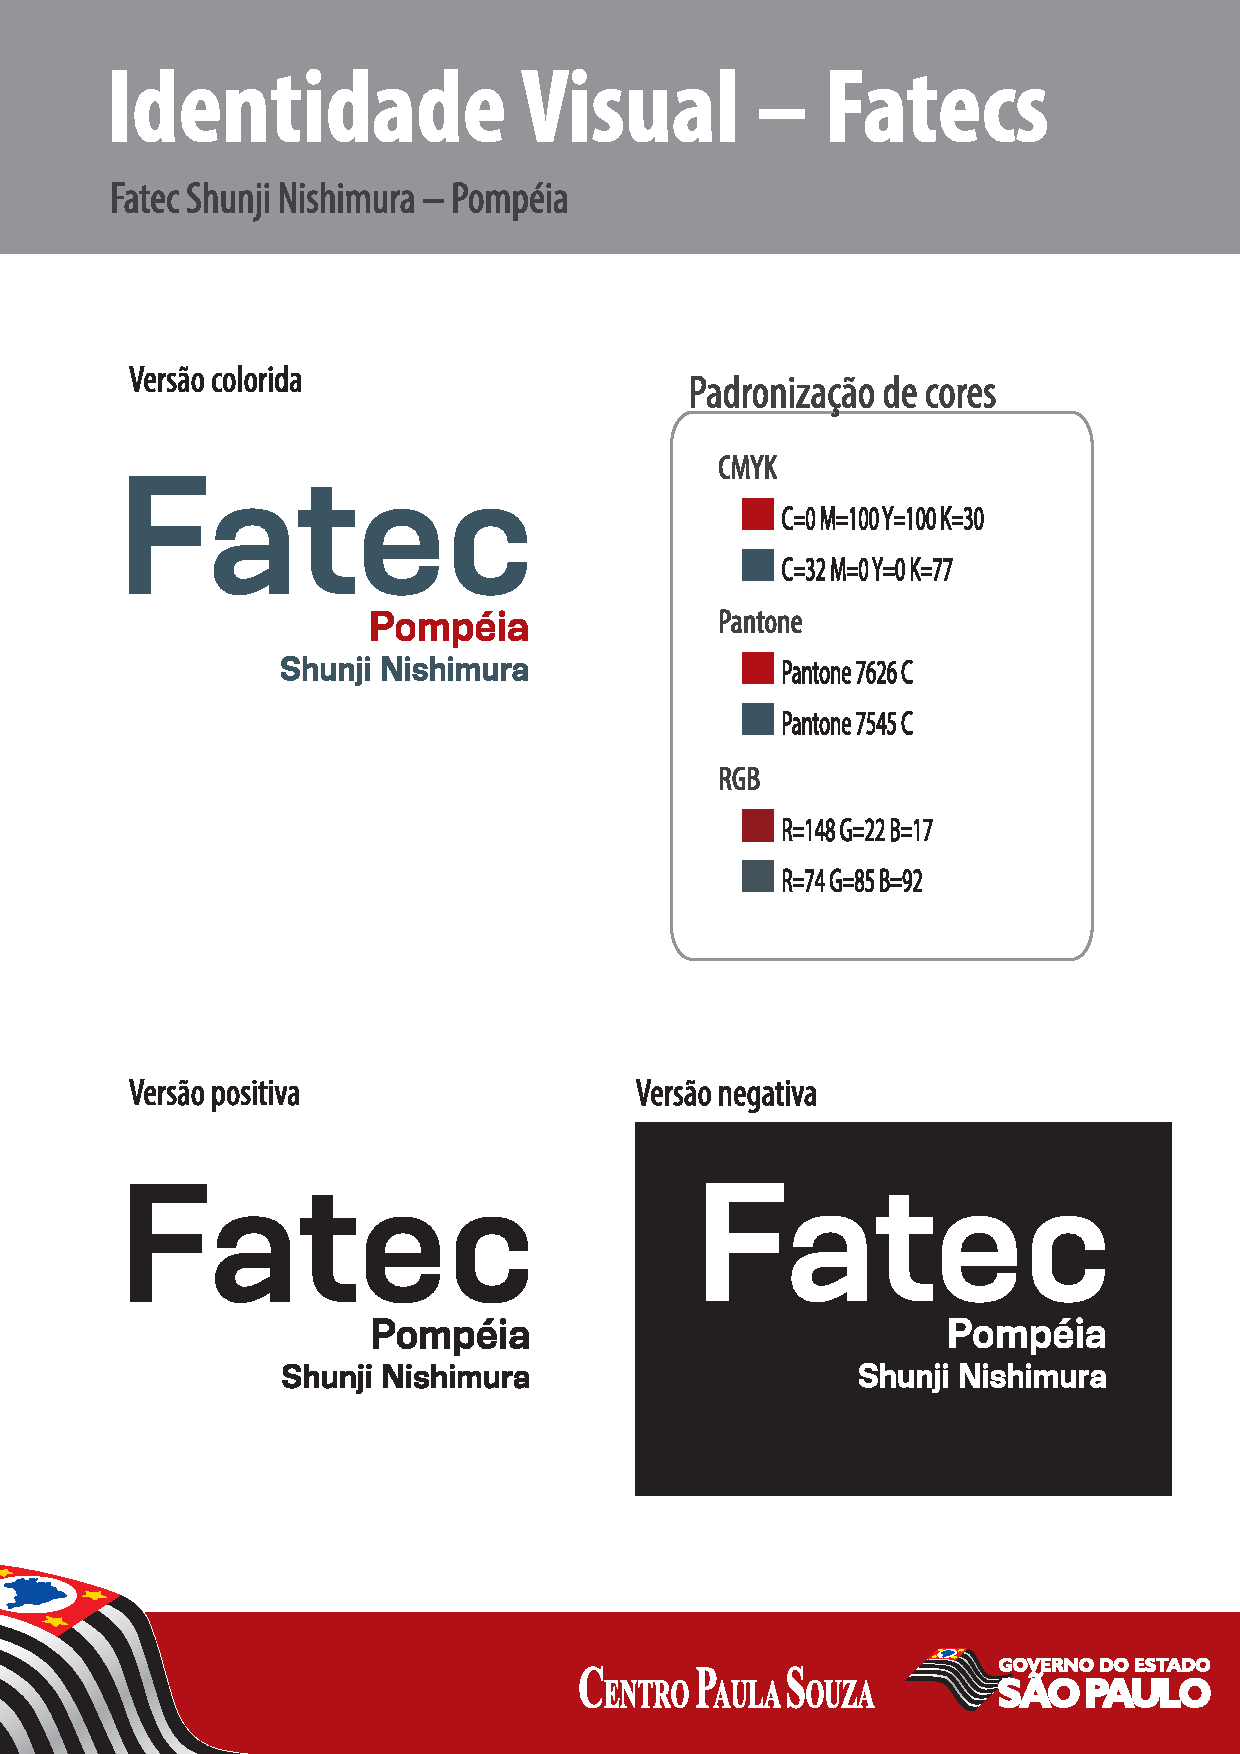
\includepdf[
    pages=-, % intervalo das páginas do arquivo pdf que serão incluídas
    scale=1, % controla o tamanho da página inserida
    pagecommand={\thispagestyle{plain} % imprime o número da página
    \refstepcounter{includepdfpage} % conta a página incluída
    \label{marcafatec.\theincludepdfpage} % marcaunb.n, n número da página
    },
    ]{fatectex-example/figuras/coresfatec}

\cleardoublepage

%\end{anexosenv}
% ---

\end{document}